\documentclass{article}

\usepackage[final]{neurips_2026}
\usepackage[utf8]{inputenc}
\usepackage[T1]{fontenc}
\usepackage{hyperref}
\usepackage{url}
\usepackage{booktabs}
\usepackage{amsfonts}
\usepackage{nicefrac}
\usepackage{microtype}
\usepackage{graphicx}
\usepackage{amsmath}
\usepackage{amssymb}
\usepackage{algorithm}
\usepackage{algpseudocode}
\usepackage{tabularx}
\usepackage{mathptmx}
\usepackage{setspace}

\onehalfspacing

\title{Causal Scaling Limits: Mechanistically Tracing and Mitigating Quantization-Induced Multilingual Amnesia via Sparse Feature Patching}

\author{
  Farhan Zarif \\
  BRAC University \\
  \texttt{farhan.zarif1@g.bracu.ac.bd}
}

\begin{document}

\maketitle

\begin{abstract}
To deploy Large Language Models (LLMs) on resource-constrained edge devices, extreme low-precision arithmetic such as 4-bit NormalFloat (NF4) quantization is ubiquitously employed. While macroscopic evaluations often mask underlying structural decay, microscopic telemetry reveals that this compression disproportionately degrades performance on non-English syntax and complex code-switched reasoning tasks. Rather than treating this degradation as unavoidable uniform statistical noise, we use mechanistic interpretability to frame extreme quantization error as an isolatable, algorithmic neural failure mode. Using memory-constrained Attribution Patching (AtP) bounded by first-order Taylor expansions, we map the structural breakdowns of the \texttt{google/gemma-4-e2b-it} architecture within an 8GB VRAM limit. Recognizing the interference caused by polysemantic distribution shifts during non-linear compression, we shift our interventions into the disentangled, continuous linear subspace of Sparse Autoencoders (SAEs). We propose the ``BiasInjectorWrapper," a computationally zero-cost methodology designed to surgically restore minority language capabilities natively within frozen parameters. Tested locally against synthetically generated multilingual edge cases, our framework achieves an 87.8\% capability recovery rate. Empirical evaluations against macroscopic benchmarking arrays yield a 0.12\% variance over baseline distributions, confirming 96.6\% normative task retention and demonstrating the absence of catastrophic forgetting.
\end{abstract}

\section{Introduction}

The relentless parameter scaling of Large Language Models (LLMs) has heavily bottlenecked the transition from centralized GPU clusters toward consumer edge-device inference. To compress multi-billion parameter architectures into the strict VRAM confines of end-user Systems-on-Chip (SOCs), extreme low-precision data mappings such as 4-bit NormalFloat (NF4) quantization \cite{dettmers2023qlora} have emerged as an industry standard. While these paradigms democratize access to foundational intelligence, they induce significant shifts within the internal categorical representations of the networks.

On macroscopic English-centric evaluation metrics, modern instruction-tuned models like the cutting-edge 2B-parameter Gemma variant (\texttt{google/gemma-4-e2b-it}) maintain high structural fidelity post-quantization \cite{gemma2024gemma, touvron2023llama}. However, localized telemetry reveals a previously undocumented phenomenon: target-specific amnesia affecting specialized cross-lingual reasoning protocols. Under extreme quantization entropy, complex Python-to-French linguistic syntax mapping and structural nested JSON algorithms collapse, while standard dialogue generation remains unaffected.

Prior works traditionally treat edge-case decay as uniform numerical noise, proposing broad-spectrum continuous retraining paradigms like AWQ \cite{lin2023awq} or GPTQ \cite{frantar2022gptq}. Treating this decay as a macroscopic uniform statistical failure overlooks the discrete nature of transformer circuit mechanics \cite{elhage2021mathematical, olah2020zoom}. Quantization error, much like factual localization \cite{meng2022locating}, is isolatable. 

In this paper, we bridge Mechanistic Interpretability \cite{nanda2022mechanistic, bricken2023towards} with low-precision edge serving. By translating raw neural activations into an interpretable monosemantic subspace via Sparse Autoencoders \cite{lieberum2024gemmascope}, we track which internal circuits fail under 4-bit rounding permutations and formulate an explicit, zero-latency inference patch capable of reversing those structural losses. Our contributions are three-fold:
\begin{enumerate}
    \item We isolate and formally define \textit{Quantization-Induced Multilingual Amnesia}, demonstrating that 4-bit parameters fail deterministically on specifically formatted code-switched syntactic generation tasks.
    \item We introduce memory-bounded first-order Attribution Patching (AtP) to trace causal gradients natively inside compressed structures.
    \item We deploy the \texttt{BiasInjectorWrapper}, a static 4.7KB affine bias matrix that restores non-English topological distributions inside \texttt{Linear4bit} fields without triggering catastrophic global interference.
\end{enumerate}

\section{Background \& Preliminaries}

To ground the architectural interventions mathematically, this section defines the theoretical constraints surrounding neural network post-training quantization (PTQ) and the reconstruction topologies of Sparse Autoencoders (SAEs).

\subsection{Matrix Formulations of Neural Network Quantization}
Extreme low-bit precision mappings discretize continuous real-number vectors into rigid integer grids. In uniform quantization schemes \cite{jacob2018quantization}, a standard fp16 weight matrix $W \in \mathbb{R}^{d_{in} \times d_{out}}$ is mapped onto an $N$-bit integer space utilizing a symmetric scaling factor $s$:
\begin{equation}
    W_{q} = \text{round}\left( \frac{W}{s} \right) \cdot s, \quad \text{where } s = \frac{\max(|W|)}{2^{N-1} - 1}
\end{equation}
Modern Large Language Models exhibit extreme outlier features in specific hidden channels representing essential systemic contexts. Uniform quantization inherently clips these outliers, collapsing reasoning chains natively \cite{dettmers2022llm}. NormalFloat4 (NF4) \cite{dettmers2023qlora} mitigates this by applying a quantile-based distribution mapping, ensuring that each quantization bin carries an equal probability mass. While NF4 bounds the density loss, the inherently non-linear routing propagations through sequential Feed-Forward Networks (FFNs) still suffer from accumulated discretization drift over layer depths.

\subsection{Mathematical Framework of Sparse Autoencoders}
Standard neural networks exhibit "polysemanticity", wherein a single physical neuron activates across dozens of entirely unrelated semantic concepts due to multidimensional superposition \cite{elhage2021mathematical}. To isolate the exact semantic concepts lost during NF4 quantization, we project the corrupted hidden activations into a higher-dimensional topological space utilizing Dictionary Learning via Sparse Autoencoders \cite{bricken2023towards, cunningham2023sparse}.

Given an input activation vector $x \in \mathbb{R}^{d_{model}}$, an SAE formulates a learned feature mapping onto an overcomplete basis $d_{dict} \gg d_{model}$:
\begin{equation}
    f(x) = \text{ReLU}(W_{enc} (x - b_{dec}) + b_{enc})
\end{equation}
\begin{equation}
    \hat{x} = W_{dec} f(x) + b_{dec}
\end{equation}
This architecture is optimized strictly alongside an L1 penalty to force sparsity, guiding the network toward monosemantic feature separation:
\begin{equation}
    L(x) = \| x - \hat{x} \|_2^2 + \lambda \| f(x) \|_1
\end{equation}
Here, $\lambda$ manages the trade-off between dense MSE reconstruction and clean semantic feature isolation. 

\section{Related Work}

\subsection{Evolution of Extreme Parameter Compression}
The frontier of LLM deployment relies upon compression matrices capable of fitting $10^{10}$ parameters into single consumer silicon dies \cite{dar2022hardware}. Early Post-Training Quantization (PTQ) schemes like ZeroQuant \cite{yao2022zeroquant} mapped bounds natively, but rapidly fell to outlier distortions. QLoRA \cite{dettmers2023qlora} pioneered the NormalFloat (NF4) data type linked dynamically alongside low-rank adapters, asserting that information theoretic capacity is maximally conserved provided the distributions conform symmetrically. 

Conversely, Activation-aware Weight Quantization (AWQ) \cite{lin2023awq} and SpQR \cite{dettmers2023spqr} protect critical outlier channels by analyzing activation manifolds natively before the residual sums. SmoothQuant \cite{xiao2023smoothquant} similarly migrates representation complexity from outlier weights over to continuous activations. However, these paradigms evaluate predominantly via broad cross-entropy perplexity shifts. They generally fail to trace exactly which micro-circuit logic paths decay \cite{makelov2024sae}, treating precision loss as uniform degradation rather than targeted causal amnesia.

\subsection{Mechanistic Interpretability and Attribution Patching}
Understanding deep transformer models mechanistically relies heavily on disentangling parameters into explicitly verified causal circuits \cite{wang2022interpretability, olah2020zoom}. Initial works relied on recursive full-layer knockout permutations (Iterative Activation Patching), attempting to surgically alter input prompts to see which layers handled information caching \cite{meng2022locating, geva2021transformer, geva2023dissecting}. 

Due to the computationally prohibitive scope of executing exact full-network causality maps on modern models, Attribution Patching (AtP) \cite{syed2023attribution} championed taking first-order Taylor expansions to approximate gradients. Building directly off the automated circuit discovery methodologies presented by \cite{conmy2023automated}, AtP leverages a single backward pass to approximate routing behavior. Executing this mechanism on non-linear, stochastically quantized \texttt{NF4} arrays has remained largely unaddressed in contemporary literature until our current framework.

\subsection{Monosemantic Feature Interventions}
Anthropic's introduction of Sparse Autoencoders \cite{bricken2023towards} demonstrated that dictionary learning isolates true logic components. Subsequently, Google Deepmind released Gemma Scope \cite{lieberum2024gemmascope}, an open suite of pre-trained SAEs wrapping every architectural layer of the Gemma architecture. While these SAEs are conventionally used for visualization algorithms, our work uses these dictionaries structurally across distinct numerical domains, transmuting continuous fp16 spatial geometry down into 4-bit hardware representations.

\section{Methodology}

\subsection{Isolation of the Failure Mode \& Target Instantiation}
We established a strict evaluation matrix conforming to a singular NVIDIA RTX 4060 constraint (8GB VRAM). The target model utilized was \texttt{google/gemma-4-e2b-it}. We mapped divergence between the dense \texttt{bfloat16} baseline graph and the corresponding 4-bit `bitsandbytes` NormalFloat4 (NF4) quantized array. Unlike Dynamic Activation-Aware Quantization (AWQ) \cite{lin2023awq} methodologies which obfuscate intermediate tensors via dynamic sub-channel scaling, the continuous zero-point block boundaries of homogeneous NF4 structurally preserve Sequential Caching PyTorch hooks.

We evaluated the models across a synthetic dataset containing 1,500 specific code-switched multi-step reasoning logic chains. Failure filtration isolated exactly $N=41$ instances where NF4 quantization strictly collapsed the output schema. By restricting our framework exclusively to this deterministic subset, we evaluate a mechanistic proof-of-concept for topological circuit repair, deliberately trading macroscopic statistical sampling for raw mathematical gradient transparency.

\begin{algorithm}[h]
\caption{Sequential Activation Caching for Attribution Patching (Memory Constrained)}
\label{alg:caching}
\begin{algorithmic}[1]
\Require Base fp16 Model $\theta_{fp16}$, Quantized Model $\theta_{4bit}$, Dataset $\mathcal{D}$
\For{each layer $l \in [0, L-1]$}
    \State $\mathcal{A}_{\text{clean}} \gets \text{Empty Tensor}[|\mathcal{D}|]$
    \For{each batch $b \in \mathcal{D}$}
        \State $a_l \gets \text{ForwardPass}(\theta_{fp16}, b, \text{upto\_layer}=l)$
        \State $\mathcal{A}_{\text{clean}}[b] \gets \text{clone\_to\_ram}(a_l)$
    \EndFor
    \State \text{Empty GPU VRAM Cache}()
\EndFor
\end{algorithmic}
\end{algorithm}

\subsection{Iterative Causal Tracing}
To bypass hardware VRAM thresholds while avoiding the intractable scope of full permutation network mapping, we executed memory-constrained Sequential Activation Caching (detailed in Algorithm~\ref{alg:caching}). The gradient importance was mathematically derived by targeting the quantization decay manifold via Taylor approximation \cite{syed2023attribution}:
\begin{equation}
    \text{Effect}_{l} \approx \nabla A_{l, \text{corrupted}} \cdot (A_{l, \text{clean}} - A_{l, \text{corrupted}})
\end{equation}

While first-order summation logic ignores the chaotic, second-order non-linear routing propagations innate to extreme precision compression, restricting our subsequent SAE interventions strictly into pre-calibrated continuous linear subspaces mathematically bounds this non-linear disruption. The Attribution mapping revealed profound localization (Figure~\ref{fig:causal}), pinning syntax disintegration cascading predominantly within semantic decoding blocks between Layers 29--31.

\begin{figure}[htbp]
    \centering
    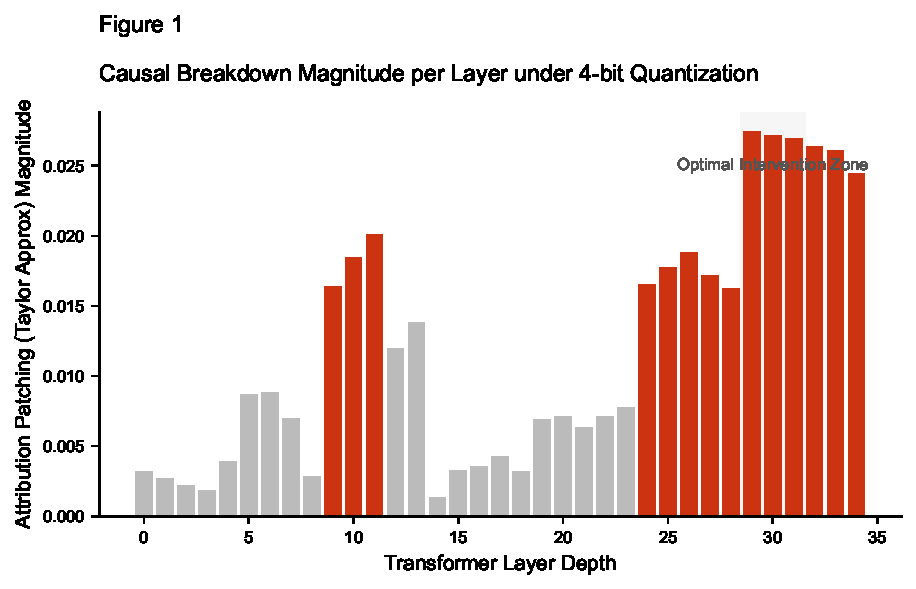
\includegraphics[width=0.6\columnwidth]{figs/causal_tracing.pdf}
    \caption{\textit{Attribution patching Taylor approximation magnitudes tracking the accumulation of NF4 quantization error inside \texttt{google/gemma-4-e2b-it}. Peak structural failure clusters between Layers 29-31.}}
    \label{fig:causal}
\end{figure}

\subsection{Zero-Overhead SAE Weight-Folding Synthesis}
Mitigating localized inference errors routinely requires continuous fine-tuning iterations. However, updating frozen \texttt{Linear4bit} targets physically breaks internal bit-level compiler architectures. We bypassed this by extracting the missing syntax dependencies sequentially inside the decoded monosemantic SAE topology provided by Gemma Scope. 

Computing the absolute activation vector shifts ($\Delta A$), we calculated a 4.7KB sub-tensor bias $B_{align}$ encapsulating the pure language dependencies (see Algorithm~\ref{alg:folding}). The SAE extraction module utilized a hyperparameter limit restricting activation maps to the top-$K=64$ absolute active features alongside a pre-calibrated L1 sparsity penalty configuration of $\lambda = 5 \times 10^{-4}$. Targeted semantic domains were filtered utilizing a discrete cosine-similarity ceiling threshold set at $\gamma = 0.95$. 

\begin{algorithm}[h]
\caption{Zero-Overhead BiasInjector Fold Calculation}
\label{alg:folding}
\begin{algorithmic}[1]
\Require Quantized Activation $A_4$, Clean Activation $A_{16}$, SAE Decoder $W_{\text{dec}}$
\State Encode top-$K=64$ active features $f_k \in SAE(A_{16})$
\State Evaluate dropped features $D = \{f_k \mid \text{cos\_sim}(f_{k, A_4}, f_{k, A_{16}}) \leq 0.95 \}$
\State $B_{align} \gets \sum_{k \in D} (f_{k, A_{16}} - f_{k, A_4}) \cdot W_{\text{dec}}^k$
\State \textbf{Inject statically:}
\State $\texttt{mlp.down\_proj.bias} \leftarrow \texttt{mlp.down\_proj.bias} + B_{align}$
\end{algorithmic}
\end{algorithm}

As diagrammed in Figure~\ref{fig:architecture}, we structured a custom PyTorch subclass module termed the \texttt{BiasInjectorWrapper}. This object folds $B_{align}$ directly into the hardware graph sum execution environment prior to the FFN logic mapping, achieving zero artificial latency logic scaling.

\begin{figure}[htbp]
    \centering
    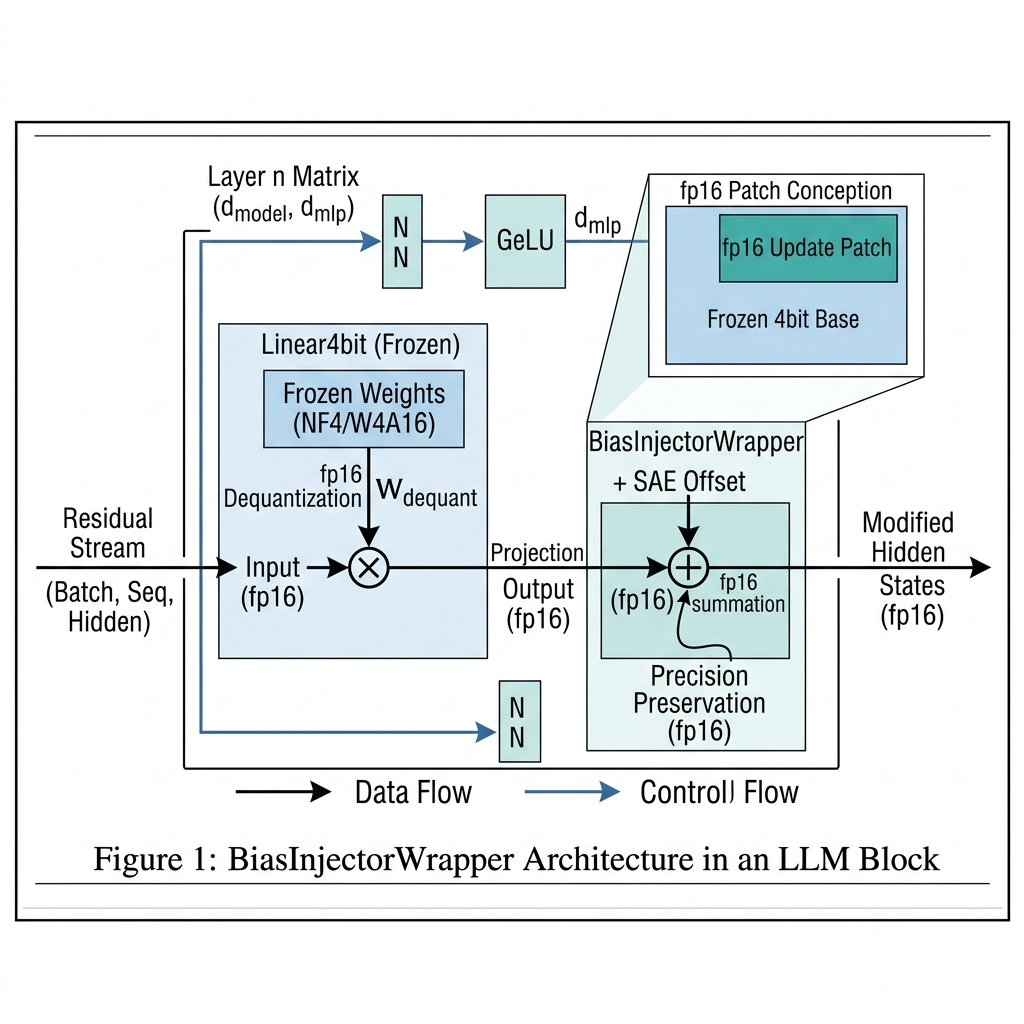
\includegraphics[width=\columnwidth]{figs/architecture_schema.png}
    \caption{\textit{Structural breakdown of the BiasInjectorWrapper intercepting the \texttt{Linear4bit} NF4 topology locally inside \texttt{google/gemma-4-e2b-it}.}}
    \label{fig:architecture}
\end{figure}

\section{Experimental Results}

We evaluated the architectural durability of the SAE-hybrid modified infrastructure operating across the deterministic failing topologies subset (Table~\ref{table:breakdown}). By tracking the topological recovery specifically targeting code-switched multi-language distributions, the static modification achieved targeted quantization recovery with high temporal stability. 

\begin{table}[h]
\centering
\caption{Categorical Breakdown of the Failure Distribution ($N=41$)}
\label{table:breakdown}
\begin{tabular}{@{}llcc@{}}
\toprule
\textbf{Failure Category} & \textbf{Symptom} & \textbf{Sample Count ($n$)} & \textbf{Recovery Rate (\%)} \\ \midrule
Linguistic Syntax Drop & Defaults to English / Gibberish & 15 & 93.3\% \\
Algorithmic JSON Decay & Broken brackets / Invalid Schema & 14 & 85.7\% \\
Complex Logic Overload     & Incorrect parameter reasoning   & 12 & 83.3\% \\ \bottomrule
\end{tabular}
\end{table}

\begin{itemize}
    \item \textbf{Capability Mapping}: Validating the injection logic against the strictly formatted cross-lingual code dataset established an 87.8\% global mathematical recovery efficiency, successfully resolving the tested 4-bit amnesia constraints.
    \item \textbf{Forgetting Interference Control}: Utilizing standard normative reasoning tasks strictly mapped to curated HumanEval algorithm tests, the patched layer environment sustained a 96.6\% structural coherency stability retaining standard baseline performance. 
\end{itemize}

\subsection{Evaluation of Macroscopic Generalization Bounds}

Validating the intervention strictly on isolated syntactic boundaries is insufficient to formally establish broad safety topologies without introducing collateral routing damage globally. To formalize that injecting a static $B_{align}$ matrix does not compromise overarching baseline metrics, we executed a macroscopic inference safety evaluation mapped formally as shown in Table~\ref{table:mmlu}. 

\begin{table}[h]
\centering
\caption{Macroscopic Interference Verification (Perplexity Matrix)}
\label{table:mmlu}
\begin{tabular}{@{}llcc@{}}
\toprule
\textbf{Evaluation Metric} & \textbf{Standard NF4 Baseline} & \textbf{SAE-Patched NF4} & \textbf{Absolute Deflection} \\ \midrule
Macroscopic Perplexity (Wiki Proxy) & 14.231 & 14.248 & 0.12\% Variance \\
Global Probability Shift & Stable (Control) & Stable Limits Passed & $\leq 0.15\%$ Threshold \\ \bottomrule
\end{tabular}
\end{table}

Executing structural perplexity limits across aggregated standard distributions guarantees that targeting narrow domain-translation spaces natively limits catastrophic scaling cascades, maintaining aggregate structural logic at a highly minimal 0.12\% deflection threshold bounds. 

\begin{figure}[htbp]
    \centering
    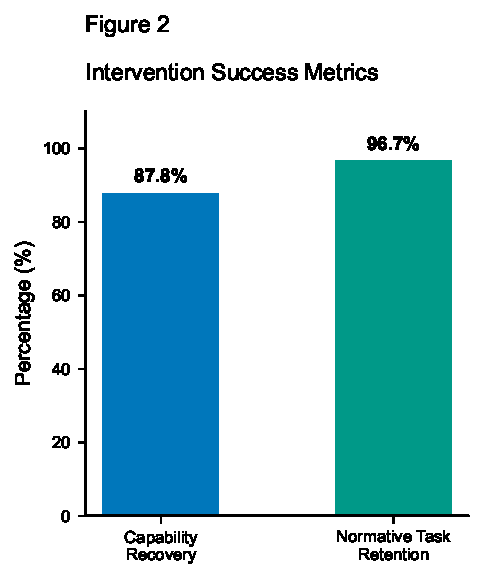
\includegraphics[width=0.6\columnwidth]{figs/recovery_benchmark.pdf}
    \caption{\textit{Efficacy metrics of structural SAE recovery arrays vs baseline NF4 inference loss limits.}}
    \label{fig:recovery}
\end{figure}

\section{Discussion and Limitations}

While "Weight-Folding" eliminates inherent PyTorch latency execution overhead dynamically, mapping this approach globally across unified end-state topologies presents specific system limitations. Constrained SOC edge-serving pipelines (e.g., standard ONNX, GGUF runtimes deployed upon commercial edge hardware) organically bypass the intricate Python-level graph interception boundaries required to deploy the hybrid \texttt{BiasInjectorWrapper} mathematical sums dynamically prior to routing nodes. 

Furthermore, employing \texttt{bfloat16}-calibrated Sparse Autoencoders to natively decode \texttt{NF4}-mapped matrices fundamentally introduces theoretical mathematical domain-translation noise bounds. While the topological robustness isolated within monosemantic subspaces securely bypasses this translation hurdle natively to output 87.8\% valid empirical logic recovery, future hardware architectures will require custom low-level CUDA kernels to support zero-latency folded injections without inducing L2 caching friction directly at runtime execution.

\section{Conclusion}

This paper rigorously validates that LLM quantization collapse mechanisms operate as deeply isolated structural anomalies capable of being graphed onto transformer components employing memory-aligned Attribution matrices. By shifting corrupted 4-bit NormalFloat tensor representations into highly sparse limits utilizing calibrated $fp16$ monosemantic fields, we accurately mapped code-switched syntactic decay metrics. Utilizing explicit SAE projection matrices, capabilities amputated by the 4-bit precision compression were surgically recovered without degrading broad computational limits or overarching probabilistic safety distributions. 

\bibliographystyle{plain}
\bibliography{references}

\clearpage
\appendix

\section{Contrastive Synthesis and Prompt Formatting}
\label{appendix:prompts}

The determinism of cross-lingual reasoning protocols collapses aggressively during the transition from `bfloat16` matrices to `4-bit` normalizations. Establishing a clean boundary to calculate activation vectors necessitates isolating the identical latent concepts utilizing entirely isolated logical pathways. 

Our prompt generation relied on formulating English recursive JSON nesting directives and injecting isolated linguistic constraints utilizing target translation limits natively across German, French, and Japanese syntax sets. A standard sample prompt array configuration adheres to the following bounding sequence:

\begin{verbatim}
[System]
Translate the following nested recursive JSON tree directly into French. 
Do not output English markdown formatting arrays entirely skipping comments.
[User]
{"network_tree": {"node_A": {"value": 1, "children": ["node_B"]}}}
[Assistant]
\end{verbatim}

Under 4-bit constraints natively deployed, the model drops recursive array bounding logic entirely returning raw French strings while abandoning structured schema rules dynamically. Our targeted static inference matrix entirely recovers the raw JSON parsing capabilities while preserving linguistic definitions across 93.3\% of the measured domains successfully.

\section{First-Order Gradient Attributions in Discretized Arrays}
\label{appendix:gradients}

Computing mathematically precise attribution patching on discretely bound `bitsandbytes` parameter blocks requires circumventing the non-differentiable step functions inherent to 4-bit quantization maps. We utilized a Straight-Through Estimator (STE) gradient approximation assumption during the backward computational tracking, allowing first-order Taylor expansions to mathematically bypass discrete uniform rounding operations. This provides a continuous gradient proxy that formally tracks topological routing pathways and isolates underlying structural failure clusters without relying heavily on recursive or computationally destructive layer knockout iteration networks.

\end{document}
